\section{Technology Assessment}
\label{sec:technology}


Introduce in (sufficient) depth the key concepts and architecture of the chosen software technology. As part if this, you may consider using a running example to introduce the technology.

This part and other parts of the report probably needs to refer to
figures. Figure~\ref{fig:framework} from \cite{brown:96} just
illustrates how figure can be included in the report.

\begin{figure}[thb]
	\centering
	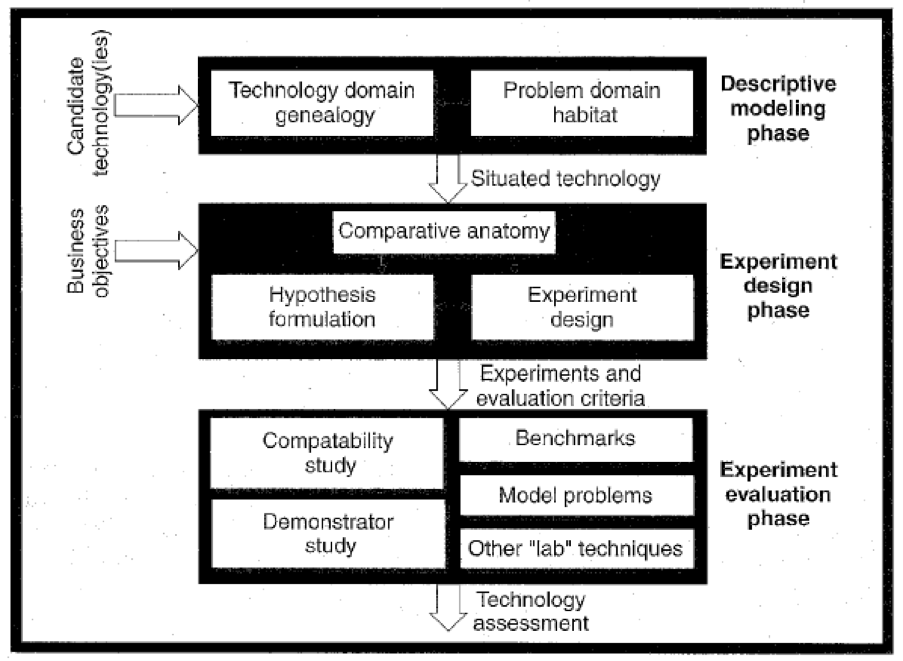
\includegraphics[scale=0.5]{figs/framework.png}
	\caption{Software technology evaluation framework.}
	\label{fig:framework}
\end{figure}

\subsection{Descriptive Modeling}

write where the technology comes from, its history, its context and what problem it solves.
Consider drawing a graph like in \cite{brown:96}.

\subsection{Experiment Design}

Write you hypotheses about what benefits the technology bring and how you can support or reject them via experiments.

\subsection{Experiment Evaluation}

Write about the results of your experiments, either via personal experience reports, quantitative benchmarks, a demostrator case study or a combination of multiple approaches.


For some reports you may have to include a table with experimental
results are other kinds of tables that for instance compares
technologies. Table~\ref{tab:results} gives an example of how to create a table.

\begin{table}[bth]
	\centering
	\begin{tabular}{llrrrrrr}
		Config & Property & States & Edges & Peak & E-Time & C-Time & T-Time
		\\ \hline \hline
		22-2 & A   &    7,944  &   22,419  &  6.6  \%  &  7 ms & 42.9\% &  485.7\% \\
		22-2 & A   &    7,944  &   22,419  &  6.6  \%  &  7 ms & 42.9\% &  471.4\% \\
		30-2 & B   &   14,672  &   41,611  &  4.9  \%  & 14 ms & 42.9\% &  464.3\% \\
		30-2 & C   &   14,672  &   41,611  &  4.9  \%  & 15 ms & 40.0\% &  420.0\% \\ \hline
		10-3 & D   &   24,052  &   98,671  & 19.8  \%  & 35 ms & 31.4\% &  285.7\% \\
		10-3 & E   &   24,052  &   98,671  & 19.8  \%  & 35 ms & 34.3\% &  308.6\% \\
		\hline \hline
	\end{tabular}
	\caption{Selected experimental results on the communication protocol example.}
	\label{tab:results}
\end{table}
